\section{Balanceo de 'arboles}

\subsection{Motivaci'on}

Intuitivamente, que un 'arbol est'e balanceado significa que no hay sub'arboles que sean mucho m'as grandes (en alg'un sentido de \textit{grande}) que otros sub'arboles. Una interpretaci'on gr'afica de esto es que un 'arbol balanceado es \textit{llano}. Los 'arboles que cumplen esta noci'on intuitiva de balanceo por excelencia, son los completos (aquellos que tienen todos los niveles completos), puesto que su altura es chica en relaci'on a la cantidad de nodos que concentra entre todos sus niveles. El hecho de que un 'arbol binario completo de $n$ nodos tiene altura aproximadamente $\lg n$, motiva la definici'on central de todo este apunte.

\begin{defi}
Un 'arbol de $n$ nodos se dice \textit{balanceado} si su altura es \Oh{\lg n}
\end{defi}

Retomando la discusi'on de la introducci'on, la utilidad pr'actica de los 'arboles balanceados aparece cuando se combina este concepto con el de 'arbol de b'usqueda. Recordemos qu'e significa esto 'ultimo.

\begin{defi}
Un 'arbol binario con claves en los nodos se dice \textit{de b'usqueda} (y escribimos ABB) si:
\begin{itemize}
	\item toda clave en el sub'arbol izquierdo es menor que la clave de la ra'iz;
	\item toda clave en el sub'arbol derecho es mayor que la clave de la ra'iz;
	\item tanto el sub'arbol izquierdo como el derecho son 'arboles binarios de b'usqueda. 
\end{itemize}
\end{defi}

Un ABB permite determinar la existencia de una clave en el 'arbol en tiempo proporcional a la altura del 'arbol \cite{cormen01}. En un ABB de $n$ nodos cualquiera, esto puede ser, en el peor caso, \Oh{n}. Sin embargo, si el 'arbol es balanceado, su altura ser'a $O(\lg n)$, con lo cual el costo de la b'usqueda baja a $O(\lg n)$.

Nuestro objetivo ser'a definir familias de 'arboles binarios que sean balanceados. Como hemos mostrado, nuestro inter'es se centra en 'arboles que puedan ser usados como estructuras de representaci'on de diccionarios, por lo que una propiedad deseada para estas familias es que al ser utilizados como ABBs, soporten la inserci'on y el borrado de nodos (es decir, la actualizaci'on a lo largo del tiempo), de modo tal que al efectuar tales operaciones se obtenga otro 'arbol de la familia de 'arboles balanceados. %Esta 'ultima propiedad es lo que nos permitir'a asegurar que a lo largo de una secuencia de operaciones, los costos de inserci'on, borrado y b'usqueda se mantienen. Esto quedar'a m'as claro y resultar'a evidente al ver ejemplos concretos.

\subsection{'Arboles binarios completos}

Como hemos visto, los 'arboles binarios completos son una familia de 'arboles balanceados elemental. El hecho de que sean balanceados se fundamenta en el siguiente resultado, al que ya hemos hecho alusi'on.

\begin{teo}
Un 'arbol binario completo $T$ de $n$ nodos tiene altura $\lg(n + 1)$.

\begin{proof}
Sea $h$ la altura de $T$. Como $T$ es completo, los $h$ niveles de $T$ est'an completos, es decir que

\[n = \sum_{i = 0}^{h - 1}2^i = 2^h - 1\]
\end{proof}
\end{teo}

\begin{coro}
Un 'arbol binario completo es balanceado.
\end{coro}

El problema con esta clase de 'arboles, es que son extremadamente r'igidos, en el sentido que no es posible realizar una inserci'on o borrado de un nodo y obtener otro 'arbol completo, como muestra la figura \ref{fig3}.

\begin{figure}[h]
	\begin{center}
	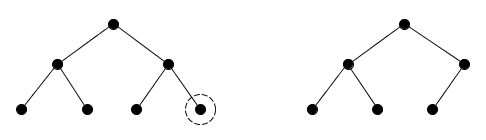
\includegraphics[scale=0.6]{imagenes/fig3.jpg}
	\end{center}
	\caption{un 'arbol binario completo deja de ser completo al eliminarle un nodo}
	\label{fig3}
\end{figure}

\subsection{Balanceo perfecto}

Necesitamos relajar un poco esta rigidez de los 'arboles completos. Observemos que una caracter'istica de un 'arbol completo es que todas sus hojas estan en el 'ultimo o en el ante'ultimo nivel. Obviamente, esta propiedad caracteriza a muchos otros 'arboles que no son completos, como muestra la figura \ref{fig1}. Para evitar casos de extremo desbalanceo, como el de la figura, pediremos que no haya nodos que tengan un s'olo hijo, que se puede ver que son los que abundan en el ejemplo, y que causan que existan ramas largas.

\begin{figure}[h]
	\begin{center}
	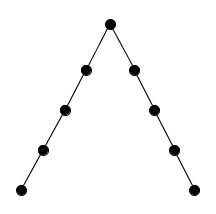
\includegraphics[scale=0.6]{imagenes/fig1.jpg}
	\end{center}
	
	\caption{'arbol que tiene sus hojas al mismo nivel, pero no es balanceado}
	\label{fig1}
\end{figure}

Con todo esto en mente, vamos a definir un nuevo criterio de balanceo, que no es m'as que una serie de restricciones sobre 'arboles binarios que definen una familia.

\begin{defi}
	Un 'arbol binario se dice \textit{lleno} si todo nodo tiene 0 o 2 hijos.
\end{defi}

\begin{defi}
	Un 'arbol binario se dice \textit{perfectamente balanceado} si:
	\begin{itemize}
		\item es un 'arbol lleno;
		\item todas sus hojas se encuentran en el 'ultimo 'o ante'ultimo nivel.
	\end{itemize}
\end{defi}

La figura \ref{fig2} muestra un 'arbol binario perfectamente balanceado. Notar que tiene forma achatada, condici'endose, intuitivamente, con la noci'on de balanceo. El siguiente resultado expresa formalmente esto 'ultimo.

\begin{figure}[h]
	\begin{center}
	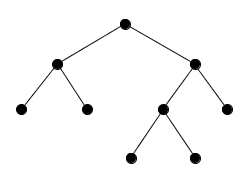
\includegraphics[scale=0.6]{imagenes/fig2.jpg}
	\end{center}
	\caption{'arbol perfectamente balanceado}
	\label{fig2}
\end{figure}

\begin{teo}
	Un 'arbol binario perfectamente balanceado $T$ de $n$ nodos tiene altura $\ceil{\lg(n + 1)}$.
\begin{proof}
	Sea $h$ la alura de $T$. Lo primero que veremos es que cada nivel $0 \leq i < h - 1$ est'a completo. En efecto, si suponemos que $i > 0$ es el primer nivel que no est'a completo, entonces existe un nodo $v$ en el nivel $i - 1$ que no tiene dos hijos, dado que el $i - 1$ est'a completo. Como $T$ es un 'arbol lleno, entonces $v$ debe tener 0 hijos, es decir que es una hoja. Luego, $T$ tiene una hoja en el nivel $i - 1 < h - 2$, lo cual contradice al hecho de que todas las hojas de dicho 'arbol est'an en el nivel $h - 1$ 'o $h - 2$.
	
	Por lo anterior, debe ser
	
	\[n > \sum_{i = 0}^{h - 2} 2^i = 2^{h - 1} - 1\]
	
	La desigualdad es estricta debido a que $T$ tiene al menos un nodo en el nivel $h - 1$.
	Por otro lado, como $T$ tiene altura $h$, se tiene
	
	\[n \leq \sum_{i = 0}^{h - 1} 2^i = 2^h - 1\]
	
	Juntando ambas desigualdades,
	
	\[2^{h - 1} - 1 < n \leq 2^h - 1\]
	
	Sumando 1 y tomando logaritmos,
	
	\[h - 1 < \lg(n + 1) \leq h\]
	
	Es decir que $h = \ceil{\lg(n + 1)}$.
	
\end{proof}
\end{teo}

\begin{coro}
	Un 'arbol binario perfectamente balanceado es balanceado.
\end{coro}

Lamentablemente, esta familia de 'arboles balanceados sigue padeciendo algunos de los problemas que tienen los 'arboles binarios completos. Particularmente sufre el problema de que no hay 'arboles perfectamente balanceados para cada cantidad de nodos posible. La figura \ref{fig4} muestra un ejemplo.

\begin{figure}[h]
	\begin{center}
	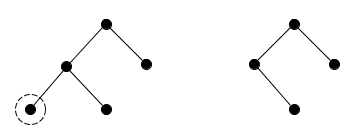
\includegraphics[scale=0.6]{imagenes/fig4.jpg}
	\end{center}
	\caption{'arbol binario perfectamente balanceado deja de ser perfectamente balanceado al eliminar un nodo}
	\label{fig4}
\end{figure}

\subsection{Balanceo en altura}

\begin{defi}
	Un 'arbol binario se dice \textit{balanceado en altura} si para cada nodo, la altura de su sub'arbol derecho e izquierdo difieren a lo sumo en una unidad.
\end{defi}

\begin{teo}
	Un 'arbol binario balanceado en altura es balanceado.
	
\begin{proof}
	La pregunta clave de la demostraci'on es,
	
	\begin{center}
	\textit{¿cu'al es la m'inima cantidad de nodos que puede tener un 'arbol binario balanceado en altura, de altura $h$?}
	\end{center}
	
	Intuitivamente, responder a esta pregunta es 'util porque fijado un 'arbol balanceado en altura de $n$ nodos y altura $h$, dicho 'arbol no puede ser demasiado ralo. Matem'aticamente, $n$ debe ser suficientemente grande,z respecto de $h$. M'as precisamente, $n$ debe estar acotado inferiormente por una funci'on de $h$. Esto se debe a que el balance deber'ia obligar a que haya una gran cantidad de nodos concentrados a lo largo de los $h$ niveles.

	%Sabiendo esto podremos acotar inferiormente a la cantidad de nodos de un 'arbol, por la cantidad m'inima de nodos que puede tener un 'arbol de su altura.
	
	Llamemos $n_{min}(h)$ a la m'inima cantidad de nodos de un 'arbol binario balanceado de altura $h$. Es claro que $n_{min}(1) = 1$ y $n_{min}(2) = 2$. Si $h > 2$, ¿cu'anto vale $n_{min}(h)$? Un 'arbol binario balanceado en altura de $n$ nodos y altura $h > 2$ debe tener dos sub'arboles, izquierdo y derecho. De la definici'on de balanceo en altura se deduce que estos dos tambi'en son balanceados en altura. Como $T$ tiene altura $h$, entonces uno de ellos tiene altura $h - 1$, y el otro altura $h - 1$ o $h - 2$, puesto que la diferencia entre las alturas de los mismos es a lo sumo 1. Gr'aficamente, la situaci'on es la siguiente:
	
\begin{figure}[H]
	\begin{center}
	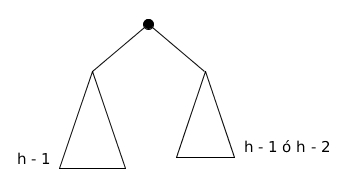
\includegraphics[scale=0.6]{imagenes/figdembh.jpg}
	\end{center}
\end{figure}

	
	Luego,
	
	\[n \geq 1 + n_{min}(h - 1) + \min(n_{min}(h - 1), n_{min}(h - 2))\]
	
Como $T$ es arbitrario de altura $h$, resulta que $n_{min}(h) \geq 1 + n_{min}(h - 1) + \min(n_{min}(h - 1), n_{min}(h - 2))$. De esta desigualdad, m'as los casos base, se sigue inmediatamente que $n_{min}(h) > n_{min}(h - 1)$ para todo $h > 1$, con lo cual la expresi'on anterior se simplifica a

\[n_{min}(h) \geq 1 + n_{min}(h - 1) + n_{min}(h - 2)\]

Para probar la igualdad, basta ver que hay alg'un 'arbol binario balanceado en altura, de altura $h$, con cantidad de nodos $1 + n_{min}(h - 1) + n_{min}(h - 2)$. Este 'arbol se puede construir f'acilmente en forma inductiva, razonando igual que antes. En definitiva,

\[n_{min}(h) = 1 + n_{min}(h - 1) + n_{min}(h - 2)\]

Observemos que esta recurrencia tiene un parecido con la sucesi'on de Fibonacci. La siguiente tabla muestra los primeros valores de $n_{min}$ y $Fib$.

\begin{center}
\begin{tabular}{|c|c|c|}
\hline
$h$ & $n_{min}(h)$ & $Fib(h)$\\
\hline
\hline
1 & 1 & 1\\
2 & 2 & 1\\
3 & 4 & 2\\
4 & 7 & 3\\
5 & 12 & 5\\
6 & 20 & 8\\
7 & 33 & 13\\
8 & 54 & 21\\
\hline
\end{tabular}
\end{center}

Queda como ejercicio para el lector probar que $n_{min}(h) = Fib(h + 2) - 1$. Dado que $Fib(k) = \Omega(\phi^k)$, tenemos $n_{min}(h) = \Omega(\phi^h)$, donde $\phi = \frac{1 + \sqrt{5}}{2}$ es el n'umero 'aureo.

Finalmente, tomemos un 'arbol binario balanceado en altura de $n$ nodos y altura $h$, y veamos que $h = O(\lg n)$. Se tiene $n \geq n_{min}(h) = \Omega(\phi^h)$, con lo cual $n = \Omega(\phi^h)$. Pero entonces $h = O(\log_{\phi} n) = O(\lg n)$.
\end{proof}
\end{teo}

Como veremos en la segunda parte de este trabajo, esta familia de 'arboles binarios balanceados ha probado ser 'util.

\subsection{Balanceo en peso}

El 'ultimo criterio de balanceo que estudiaremos no es una propuesta superadora del balanceo en altura. A'un as'i, es interesante conocerlo, sencillamente con el fin de reforzar la idea de que hay diversas propiedades que se le pueden exigir a un 'arbol de manera tal de asegurar su balance, aunque no todas son igualmente 'utiles debido a su mayor o menor flexibilidad.

\begin{defi}
	Un 'arbol se dice \textit{balanceado en peso} si para cada nodo, la cantidad de nodos en su sub'arbol derecho e izquierdo difieren a lo sumo en una unidad.
\end{defi}

\begin{teo}
	Un 'arbol binario balanceado en peso $T$ de $n$ nodos tiene altura $\ceil{\lg(n + 1)}$.

\begin{proof}
	Sea $h$ la altura de $T$. Veamos, primero, que al igual que los 'arboles binarios perfectamente balanceados, esta clase de 'arboles tienen cada nivel $0 \leq i < h - 1$ completo. Procedemos por inducci'on en $h$.
	El caso $h = 1$ es trivial. Sea $h > 1$. Sea $r$ la ra'iz de $T$. Si $r$ tiene un 'unico hijo entonces $T$ s'olo puede estar compuesto por $r$ y su hijo, puesto que es balanceado en peso, con lo cual vale el resultado. Supongamos que $r$ tiene dos hijos. Entonces, $r$ tiene un sub'arbol izquierdo $L$ y uno derecho $R$, con alturas $h_L$ y $h_R$ respectivamente, y tama\~nos $n_L$ y $n_R$ respectivamente. Gr'aficamente este 'arbol tiene la siguiente forma:
	
\begin{figure}[H]
	\begin{center}
	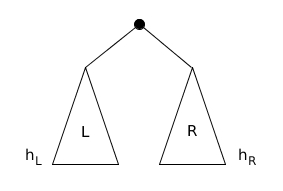
\includegraphics[scale=0.6]{imagenes/figdembp.jpg}
	\end{center}
\end{figure}

	Como $T$ es balanceado, se tiene
	
\begin{equation}
	|n_R - n_L| \leq 1	
\end{equation}

	M'as a'un, tanto $L$ como $R$ son balanceados en peso. Como adem'as ambos tienen altura menor que $h$, vale la hip'otesis inductiva sobre ellos, con lo cual $L$ y $R$ tienen todo nivel completo, excepto, quiz'as, el 'ultimo.
	
	Como $T$ tiene altura $h$ entonces podemos suponer, sin p'erdida de generalidad, que $h_L = h - 1$. Como $L$ tiene los primeros $h - 2$ niveles completos, vale
	
\[n_L > \sum_{i = 0}^{h - 3} 2^i = 2^{h - 2} - 1\]

	La desigualdad es estricta porque $L$ tiene al menos un nodo en el nivel $h - 2$. En definitiva

\begin{equation}
	n_L \geq 2^{h - 2}
\end{equation}	

	 De la ecuaci'on (1) se deduce que $n_R \geq n_L - 1$. Juntando esto con (2) resulta que 

\begin{equation}
	n_R \geq 2^{h - 2} - 1
\end{equation}	
	
	Como $R$ tiene altura $h_R$, entonces $n_R \leq 2^{h_R - 1} - 1$. Combinando esto 'ultimo con (3),
	
\[2^{h - 2} - 1 \leq 2^{h_R - 1} - 1\]

Luego $h_R \geq h - 1$, pero como $h_R$ tiene altura a lo sumo $h - 1$, debe ser $h_R = h - 1$. En definitiva, ambos sub'arboles de $r$ tienen la misma altura $h - 1$ y tienen todos sus niveles completos, salvo quiz'as el 'ultimo, lo cual prueba lo que quer'iamos y concluye la inducci'on.

A partir de aqu'i se procede igual que en el caso del balanceo perfecto.

\end{proof}
\end{teo}